\documentclass[t]{beamer}

\usepackage[english]{babel}

\usepackage{tikz}
\usepackage{setspace}
\usepackage[utf8]{inputenc}
\usepackage[TS1,T1]{fontenc}
\usepackage{csquotes}
\usepackage{pgfpages}
\usepackage{listings}
\usepackage{textcomp}
\usepackage{multirow}
\usepackage{textpos}

\usepackage[backend=biber,isbn=false,doi=false,url=false,maxcitenames=99,giveninits=true]{biblatex}

\usepackage{pgfplots}

\usepackage{tikz}
  \usetikzlibrary{positioning}
  \usetikzlibrary{tikzmark} % arrows in tex
  \usetikzlibrary{arrows}   % arrows in tex
  \usetikzlibrary{calc}     % (node)+(3cm,2cm)
  \tikzstyle{every picture}+=[remember picture]

\addbibresource{references.bib}

\usetheme[english, titlepage0]{KIT}
\setbeamercovered{transparent}

\setbeamertemplate{enumerate items}[circle]	% ball

\def\thisauthor{Simon Korz}
\def\email{uhelj@student.kit.edu}

\title{Improving Usability and Reliability of an IoT-based Controller for a Coffee Machine}
\date{20-03-2020}

\subtitle{\thisauthor{} \textendash{} \email}
\author{\thisauthor}
\institute[\raisebox{-3.5mm}{\includegraphics[height=\KITlogoht]{CES-Logo.png}}]{CES - Chair for Embedded Systems}
\logo{\includegraphics[width=\KITlogowd]{CES-Logo.png}}
\TitleImage[height=\titleimageht]{ces_title.jpg}

\newcommand{\btVFill}{\vskip0pt plus 1filll}

% \setbeameroption{show notes on second screen=right}
% \setbeameroption{second mode text on second screen} % um Videos auf notizseiten zu verhindern
% \setbeameroption{show notes}

\begin{document}

\maketitle


% \begin{frame}{Introduction}
%     \begin{columns}
%         \begin{column}[t]{0.4\textwidth}
%             \begin{itemize}
%                 \item Foo
%             \end{itemize}	
%         \end{column}
%         \begin{column}[t]{0.55\textwidth}
%             \begin{figure}
%                 \centering
%                 \includegraphics[width=\linewidth]{CES-Logo.png}
%             \end{figure}
%         \end{column}
%     \end{columns}
% \end{frame}	
\begin{frame}{Introducing the Topic}
    \begin{tikzpicture}
    \node[inner sep=0pt] (cm) at (0,0)
    {\includegraphics[width=.2\textwidth]{images/coffeeMachine.png}};
    \node[inner sep=0pt] (pi) at (5,0)
    {\includegraphics[width=.25\textwidth]{images/raspberry.jpg}};
    \node[inner sep=0pt] (rfid) at (9,0)
    {\includegraphics[width=.2\textwidth]{images/rfid.jpg}};
    \node[inner sep=0pt,outer sep=2pt] (buzzer) at (5,-2.5)
    {\includegraphics[width=.1\textwidth]{images/LK-Buzzer-1.png}};
    \node[rectangle,draw] (tag) at (9,-2.0) {RFID tag};
    \node[inner sep=0pt] (touch) at (5,2.5)
    {\includegraphics[width=.2\textwidth]{images/touchscreen.png}};
    \node[inner sep=0pt] (screen) at (5,2.93)
    {\includegraphics[width=.15\textwidth]{../thesis/images/order_page.png}};
    \node[rectangle,rounded corners,draw,fill=KITgreen50,align=center,outer sep=2pt] (server) at (9,2.5) {Accounting \\ Server};

    \path[thick,fill=green]
    (pi) edge [<-] node {} (rfid)
    edge [<->] node {} (touch)
    edge [->] node {} (buzzer)
    edge [<->] node[right=1mm] {HTTP} (server)
    edge [<->] node[fill=white,rectangle,draw,align=left] {Adapter \\ Board} (cm)
    (rfid) edge [<-] (tag)
    ;
\end{tikzpicture}
\end{frame}

\begin{frame}{Goals}
    Solve existing issues in previous system:
    \begin{itemize}
        \item Fixing bugs
        \item Redesigning the UI
        \item Adding missing features
    \end{itemize}
    \vspace*{1em}
    \begin{center}
        \textbf{$\rightarrow$ improve usability and reliability}
    \end{center}
\end{frame}

\begin{frame}{Structure of this Talk}
    \tableofcontents
    % \btVFill
    % \begin{center}
    %     \textbf{something}
    % \end{center}
    % \btVFill
    % \note{notetakingtested}
\end{frame}

\section{Introduction}
\begin{frame}{Part 1}
    \Huge\textbf{Introduction}
\end{frame}

\begin{frame}{The Components}
    \begin{tikzpicture}
    \node[inner sep=0pt] (cm) at (0,0)
    {\includegraphics[width=.2\textwidth]{images/coffeeMachine.png}};
    \node[inner sep=0pt] (pi) at (5,0)
    {\includegraphics[width=.25\textwidth]{images/raspberry.jpg}};
    \node[inner sep=0pt] (rfid) at (9,0)
    {\includegraphics[width=.2\textwidth]{images/rfid.jpg}};
    \node[inner sep=0pt,outer sep=2pt] (buzzer) at (5,-2.5)
    {\includegraphics[width=.1\textwidth]{images/LK-Buzzer-1.png}};
    \node[rectangle,draw] (tag) at (9,-2.0) {RFID tag};
    \node[inner sep=0pt] (touch) at (5,2.5)
    {\includegraphics[width=.2\textwidth]{images/touchscreen.png}};
    \node[inner sep=0pt] (screen) at (5,2.93)
    {\includegraphics[width=.15\textwidth]{../thesis/images/order_page.png}};
    \node[rectangle,rounded corners,draw,fill=KITgreen50,align=center,outer sep=2pt] (server) at (9,2.5) {Accounting \\ Server};

    \path[thick,fill=green]
    (pi) edge [<-] node {} (rfid)
    edge [<->] node {} (touch)
    edge [->] node {} (buzzer)
    edge [<->] node[right=1mm] {HTTP} (server)
    edge [<->] node[fill=white,rectangle,draw,align=left] {Adapter \\ Board} (cm)
    (rfid) edge [<-] (tag)
    ;
\end{tikzpicture}
\end{frame}

\begin{frame}{System Details}
    \begin{itemize}
        \item Broadcom BCM2837, 4 core Cortex-A53 (ARMv8) 64-bit SoC @ 1.2GHz
        \item 1GB LPDDR2 SDRAM
        \item OS: Raspbian GNU/Linux (Debian 10 Buster)
        \item Language: Python
        \item GUI: PyQt5 Framework
    \end{itemize}
\end{frame}

\begin{frame}{Available Sensors}
    \begin{textblock}{5}(8,7)
        \huge adapter board connected via \textcolor{KITgreen}{GPIO}
    \end{textblock}
    \begin{itemize}
    \item\textbf{water flow}\\
    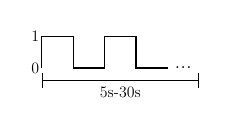
\begin{tikzpicture} [
            scale=0.4, every node/.style={scale=0.4}, yshift=-10
        ]
        % \clip (-0.1,-0.7) rectangle (4,1.1);
        \draw[] (0,0) -- (0,1) -- (1,1) -- (1,0) -- (2,0)
        -- (2,1) -- (3,1) -- (3,0) -- (4,0);
        \node[font=\huge] at (4.5, 0) {...};
        \node[font=\Large] at (-0.2,0) {0};
        \node[font=\Large] at (-0.2,1) {1};
        \path[|-|,font=\Large] (0,-0.4) edge node[below=1pt]{5s-30s} (5,-0.4);
    \end{tikzpicture}\\
    variable frequency, proportional to flow speed
    \btVFill
    \item\textbf{grinder}\\
    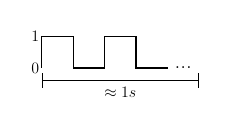
\begin{tikzpicture} [
            scale=0.4, every node/.style={scale=0.4}, yshift=-10
        ]
        % \clip (-0.1,-0.7) rectangle (4,1.1);
        \draw[] (0,0) -- (0,1) -- (1,1) -- (1,0) -- (2,0)
        -- (2,1) -- (3,1) -- (3,0) -- (4,0);
        \node[font=\huge] at (4.5, 0) {...};
        \node[font=\Large] at (-0.2,0) {0};
        \node[font=\Large] at (-0.2,1) {1};
        \path[|-|,font=\Large] (0,-0.4) edge node[below=1pt]{$\approx 1s$} (5,-0.4);
    \end{tikzpicture}\\
    variable frequency
    \btVFill
    \item\textbf{water level/blocking}\\
        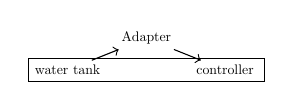
\begin{tikzpicture}[
                      scale=0.5, every node/.style={scale=0.5}
                  ]
                  \node at (0,0) (wt) {water tank};
                  \node at (2,0.8) (pi) {Adapter};
                  \node at (4,0) (ctrl) {controller};
                  % \node[rectangle,draw,minimum size=(4mm,8mm)] at (0,0){};
                  % \draw[] (wt) -- (1.5,0) -- (2.5,0.4) (2.5,0) -- (3.5,0);
                  \draw[->] (wt) -- (pi);
                  \draw[->] (pi) -- (ctrl);
                  \draw (-1,-0.3) rectangle +(6,0.6);
                  % \node[fill=black,circle,draw,inner sep=1pt] at (1,0){};
              \end{tikzpicture}\\
     input AND output
    \end{itemize}
\end{frame}

\begin{frame}{Accounting Server}
    Treasury, keeps record of
    \begin{itemize}
        \item Transactions (withdrawals, deposits, coffee bought)
        \item Users
        \item RFIDs
    \end{itemize}

    \vspace*{2em}
    Technical:
    \begin{itemize}
        \item Dedicated server, local network
        \item MySQL database
        \item Apache + PHP webserver
        \item Account balance results from accumulating all transaction deltas
    \end{itemize}
\end{frame}



\begin{frame}{Usability \& Reliability}
    Usability is the "extent to which a system, product or service can be \\
    \vspace*{0.8em}
    used by \textcolor{KITgreen}{specified users} \\
    \vspace*{0.8em}
    to achieve \textcolor{KITgreen}{specified goals} \\
    \vspace*{0.8em}
    with
    \begin{itemize}
        \item \textcolor{KITgreen}{effectiveness}
        \item \textcolor{KITgreen}{efficiency}
        \item \textcolor{KITgreen}{satisfaction}
    \end{itemize}
    \vspace*{0.8em}
    in a \textcolor{KITgreen}{specified context of use}" \scriptsize [ISO 9241-11:2018] \normalsize \\
    \rule{4cm}{0.4pt} \\
    \vspace*{.5em}
    Reliability
    \begin{itemize}
        \item Result of usability
        \item High availability
    \end{itemize}
\end{frame}

\section{Problem Analysis}
\begin{frame}{Part 2}
    \Huge\textbf{Problem Analysis}
\end{frame}
\begin{frame}{21 Issues Identified}
    \begin{itemize}
        \item GUI related
              \begin{itemize}
                  \item Size of controls
                  \item Focus on information
                  \item Timeouts
              \end{itemize}
        \item Bugs
              \begin{itemize}
                  \item Application unresponsive/freezing
                  \item Coffee not registered or recognized as hot water
                  \item Offline orders not synchronized
                  \item High CPU usage
              \end{itemize}
        \item Missing features
              \begin{itemize}
                  \item Support for new KIT-Card
                  \item Dispensing limit for consumption
                  \item Various buzzer sounds
                  \item 3D-printed case
              \end{itemize}
              % \item GUI01 Bad visibility of important information
              % \item GUI02 Milk preference controls to small
              % \item GUI03 Saving milk preferences not working
              % \item GUI04 Entertainment content is not working
              % \item GUI05 Information for unknown RFID tag disappears to fast
              % \item GUI06 Screensaver confuses users and fails to show if water is empty or not
              % \item BUG01 Coffee recognized as hot water
              % \item BUG02 Rinsing after wake up charges the user with hot water
              % \item BUG03 The GUI freezes regularly, requiring a restart
              % \item BUG04 Free coffee when water tank is refilled
              % \item BUG05 Free coffee when canceling while coffee is ground
              % \item BUG06 Offline mode not functional
              % \item BUG07 RFID reader not responsive
              % \item BUG08 3D-Model not printable
              % \item F01 No support for new KIT-Card
              % \item F02 High CPU usage
              % \item F03 Warm-up requires the user to log in several times
              % \item F04 Logging not sufficient
              % \item F05 Text files are used for IPC
              % \item F06 Buzzer has only one sound
              % \item F07 The system has poor code quality that makes it hard to maintain
    \end{itemize}
\end{frame}

\begin{frame}{GUI Problems}
    \scriptsize{Screenshot from previous system}
    \includegraphics[width=0.98\textwidth]{../thesis/images/order-page-v2.png}
\end{frame}


\begin{frame}{Reading GPIO + Managing State + IPC}
    \begin{figure}[h]
        \centering
        \includegraphics[trim={0cm 1mm 0cm 0cm},clip,width=\textwidth]{./images/code.png}
    \end{figure}
\end{frame}

\begin{frame}{Unfinished Case}
    \footnotesize{Top part of previous model}
    \includegraphics[width=\textwidth]{../thesis/images/case-top-annotated.png}
\end{frame}

\section{New Design \& Architecture}
\begin{frame}{Part 3}
    \Huge\textbf{New Design \& Architecture}
\end{frame}

\begin{frame}{New GUI}
    \begin{itemize}
        \item Focus on important information
        \item Large buttons, suitable for touch
        \item Visual feedback for each step in ordering process
    \end{itemize}
    \btVFill
    \begin{center}
        \includegraphics[width=0.7\textwidth]{../thesis/images/gui-new-1.png}
    \end{center}
\end{frame}

\begin{frame}<1-10>{The State Machine}
    \setbeamercovered{invisible}
    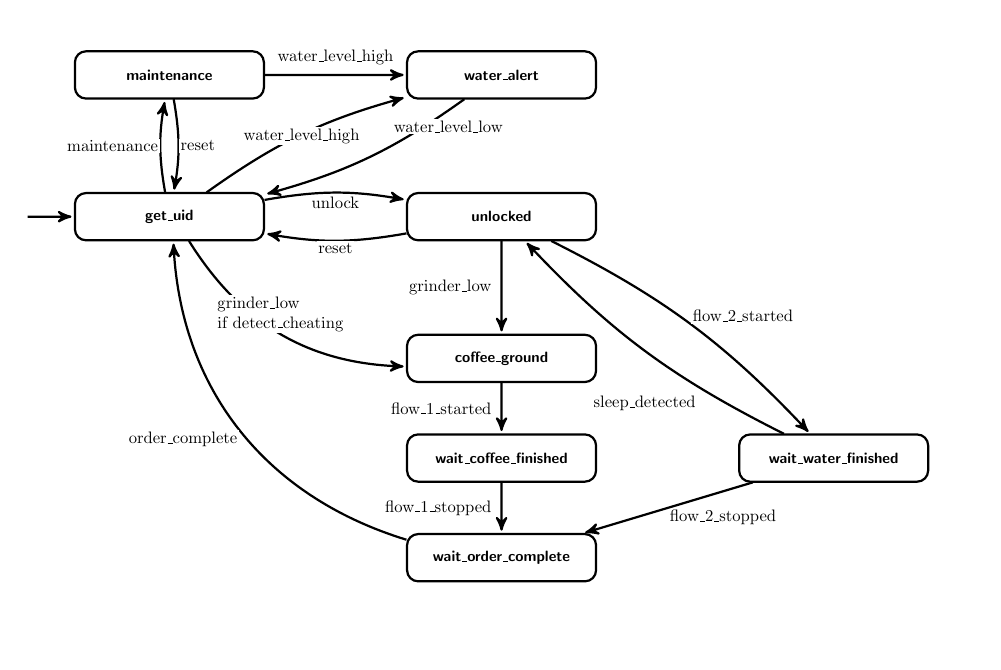
\begin{tikzpicture}[->,>=stealth',shorten >=1pt,auto,node distance=3cm,
            thick,main node/.style={rectangle,rounded corners,draw,
                    font=\sffamily\small\bfseries,minimum width=40mm,minimum height=10mm},
            empty node/.style={inner sep=0, outer sep=0},
            scale=0.6,every node/.style={scale=0.6,fill=white,inner sep=1pt}
        ]
        \clip (-3,-12) rectangle (17,1);
        % \draw[gray,step=0.25] (-3,-10) grid (10, 1);
        \uncover<2->{\node[main node] (mtn) [] {maintenance};}
        \uncover<1->{\node[main node] (gu) [below of=mtn] {get\_uid};}
        \uncover<4->{\node[main node] (ul) [right of=gu,node distance=20em] {unlocked};}
        \uncover<3->{\node[main node] (wa) [above of=ul] {water\_alert};}
        \uncover<5->{\node[main node] (cg) [below of=ul] {coffee\_ground};}
        \uncover<6->{\node[main node] (wcf) [below of=cg,node distance=6em] {wait\_coffee\_finished};}
        \uncover<9->{\node[main node] (wwf) [right of=wcf,node distance=20em] {wait\_water\_finished};}
        \uncover<7->{\node[main node] (woc) [below of=wcf,node distance=6em] {wait\_order\_complete};}
        \node[empty node] (start) [left=of gu] {};
        % \node[empty node] (other1) [above of=ul,node distance=5em] {};
        % \node[empty node] (other2) [above of=gu,node distance=5em] {};

        \draw (mtn) edge node[above=1mm]{water\_level\_high} (wa);

        \uncover<1->{\draw
            (start) edge node {start} (gu)
            ;}
        \uncover<2->{\draw
            (gu) edge [bend left=10] node {maintenance} (mtn)
            (mtn) edge [bend left=10] node {reset} (gu)
            ;}
        \uncover<3->{\draw
            (wa) edge [bend left=10] node[above right=4mm] {water\_level\_low} (gu)
            (gu) edge [bend left=10] node[below=-1mm]{water\_level\_high} (wa)
            ;}
        \uncover<4->{\draw
            (gu) edge [bend left=10] node[below=0.2mm] {unlock} (ul)
            (ul) edge[bend left=10] node[] {reset} (gu)
            ;}
        \uncover<5->{\draw
            (ul) edge [] node[left=1mm] {grinder\_low} (cg)
            ;}
        \uncover<6->{\draw
            (cg) edge [] node[left=1mm] {flow\_1\_started} (wcf)

            ;}
        \uncover<7->{\draw
            (wcf) edge [] node[left=1mm] {flow\_1\_stopped} (woc)
            (woc) edge [bend left=35] node {order\_complete} (gu)
            ;}
        \uncover<8->{\draw
            (gu) edge [bend right=28] node[align=left, above=0mm]{grinder\_low \\ if detect\_cheating} (cg)
            ;}
        \uncover<9->{\draw
            (ul) edge [bend left=10, yshift=-3pt] node {flow\_2\_started} (wwf)
            (wwf) edge [] node {flow\_2\_stopped} (woc)
            ;}
        \uncover<10->{\draw
            (wwf) edge [bend left=10] node[below=5.5mm] {sleep\_detected} (ul)
            ;}

        % \path[every node/.style={font=\sffamily\scriptsize,
        %             fill=white,inner sep=1pt}]
        % %   % Right-hand-side arrows rendered from top to bottom to
        % %   % achieve proper rendering of labels over arrows.
        % %   (M) edge [loop above] node {PrRd/-, PrWr/-} (M)
        % % (start) edge node {start} (gu)


        % %  edge [] node[left=1mm] {unlock} node[right=1mm] {grinder\_low if detect\_cheating} (ul)




        % ;

    \end{tikzpicture}
\end{frame}

\begin{frame}{Leveraging Multiple CPU Cores}
    \begin{columns}[T]
        \begin{column}{0.34\textwidth}
            \begin{itemize}
                \item 4 cores available
                \item Bidirectional pipes
                \item Predefined messages e.g,
                      CMD\_PAUSE, CMD\_RESUME, CMD\_LOCK, E\_GOT\_ID
            \end{itemize}
        \end{column}
        \begin{column}{0.6\textwidth}
            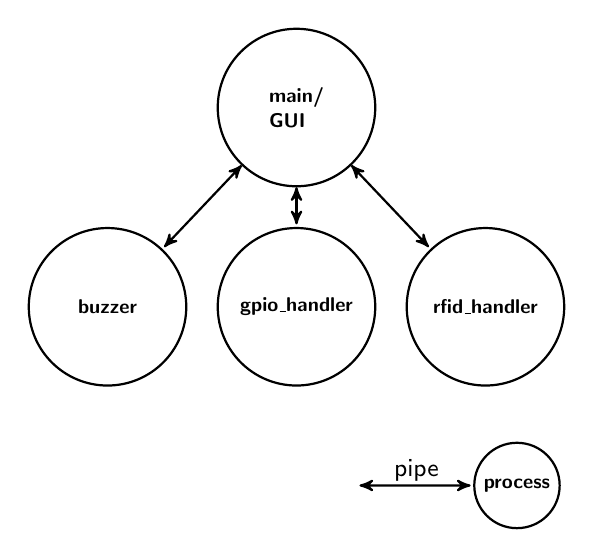
\begin{tikzpicture}[<->,>=stealth',shorten >=1pt,auto,node distance=3cm,
                    thick,main node/.style={circle,draw,
                            font=\sffamily\small\bfseries,minimum width=25mm,minimum height=10mm},
                    empty node/.style={inner sep=0, outer sep=0},
                    scale=0.8,every node/.style={scale=0.8}]

                \node[main node, align=left] (main) {main/ \\ GUI};
                \node[main node] (gpio) [below of=main, node distance=9em] {gpio\_handler};
                \node[main node] (rfid) [right of=gpio] {rfid\_handler};
                \node[main node] (buzzer) [left of=gpio] {buzzer};
                \node[main node,minimum width=5mm, minimum height=5mm] (ps) at (3.5,-6) {process};

                \path[every node/.style={font=\sffamily\small,
                            fill=white,inner sep=1pt}]
                (main) edge [] node {} (gpio)
                edge [] node[left=1mm] {} node[right=1mm] {} (rfid)
                edge [] node {} (buzzer)

                (1,-6) edge[] node{pipe} (ps)
                ;
            \end{tikzpicture}
        \end{column}
    \end{columns}
\end{frame}

\begin{frame}{Changes in GPIO Handling}
    \huge
    \begin{itemize}
        \item \textbf{\textcolor{KITgreen}{Callbacks}} instead of \textbf{\textcolor{KITgreen}{polling}}
        \item Using pigpio library instead of RPi.GPIO
              \begin{itemize}
                  \item Supports callbacks through hardware interrupts
                  \item Noise filters
              \end{itemize}
    \end{itemize}
\end{frame}

\begin{frame}{3D-Printed Case}
    \begin{itemize}
        \item Designed with Blender
        \item Stereolithography printer, resin fluid hardened by laser
        \item Challenges: Non-manifold geometry i.e. "not watertight", \\walls too thin/unstable, characteristics of the material
    \end{itemize}
    \begin{center}
        \includegraphics[trim={5cm 1cm 2.5cm 2.4cm},clip,width=0.48\textwidth]{../thesis/images/new-front.png}
        \includegraphics[width=0.48\textwidth]{../thesis/images/new-rear-bottom.png}
    \end{center}
\end{frame}

\section{Results}
\begin{frame}{Part 4}
    \Huge\textbf{Results}
\end{frame}

\begin{frame}{Printing Costs}
    \begin{itemize}
        \item Resin tank: €65.45
        \item 1L grey resin: €160.65
    \end{itemize}
    \vspace*{1em}
    \[\frac{\text{resin tank €}65.45 + \text{resin €}160.65}{1000 ml} = \text{€}0.2261/ml\]
    \begin{itemize}
        \item Top part: 90.79ml => €20,53
        \item Bottom part: 150.08ml => €33.93
        \item Screen frame: 53.60+ml => €12.12
        \item Total €66.58
    \end{itemize}
    \btVFill
    \begin{center}
        \textbf{Total cost estimate incl. prototypes > €300}
    \end{center}
    \btVFill
\end{frame}

\begin{frame}{Reduced CPU Usage}
    Measurements made with \texttt{ps} command one hour after boot \newline{}
    \vspace*{1em}
    \vskip0pt plus 1fil
    % \begin{tabular}{lrrl}
    %     \hline
    %      & \%CPU & \%memory & python module                 \\
    %     \hline
    %     \multirow{4}{*}{Old}
    %      & 98.1  & 1.8      & inputGPIO.py (GPIO \& buzzer) \\
    %      & 12.4  & 2.1      & inputGPIO.py (RFID)           \\
    %      & 0.1   & 10.2     & main.py (GUI)                 \\
    %      & 0.0   & 1.6      & inputGPIO.py (locking)        \\
    %     \hline \hline
    %     \multirow{5}{*}{New}
    %      & 5.9   & 0.1      & pigpiod (GPIO)                \\
    %      & 16.3  & 3.9      & main.py (RFID)                \\
    %      & 0.7   & 10.6     & main.py (GUI)                 \\
    %      & 0.4   & 4.6      & main.py (GPIO \& locking)     \\
    %      & 0.0   & 4.4      & main.py (buzzer)              \\
    %     \hline
    % \end{tabular}
    \begin{tabular}{lrl}
        \hline
         & \%CPU & python module                 \\
        \hline
        \multirow{4}{*}{Old}
         & 98.1  & inputGPIO.py (GPIO \& buzzer) \\
         & 12.4  & inputGPIO.py (RFID)           \\
         & 0.1   & main.py (GUI)                 \\
         & 0.0   & inputGPIO.py (locking)        \\
        \hline \hline
        \multirow{5}{*}{New}
         & 5.9   & pigpiod (GPIO)                \\
         & 16.3  & main.py (RFID)                \\
         & 0.7   & main.py (GUI)                 \\
         & 0.4   & main.py (GPIO \& locking)     \\
         & 0.0   & main.py (buzzer)              \\
        \hline
    \end{tabular}

    \scriptsize \% CPU is the ``cpu utilization of the process in "\#\#.\#" format.
    Currently, it is the CPU time used divided by the time the process has been running (cputime/realtime ratio),
    expressed as a percentage." [ps(1) manpage]
    % \% memory is the ``ratio of the process's resident set size  to the
    % physical memory on the machine, expressed as a
    % percentage." 
\end{frame}

\begin{frame}{The (Almost) Final System}
    \includegraphics[trim={0cm 48cm 2cm 29cm},clip,width=\textwidth]{./images/final-picture.jpg}
\end{frame}

\begin{frame}{Conclusion}
    \textbf{21/21 issues resolved}\\
    However: Occasionally coffee brewed without grinder signal \\ But: workaround in place
    \btVFill
    \begin{itemize}
        \item \textbf{18/21 issues directly address usability}
        \item Removed bugs, increased reliability
        \item System observed to run for 1 month without restart
              % \item Positive user feedback
        \item Offline mode
        \item Dispensing limit
        \item Better handling of warm up
    \end{itemize}
    \vspace*{1em}
    \btVFill
    \textbf{$\rightarrow$ goal of improving usability and reliability accomplished}
\end{frame}

\begin{frame}{3D-Printed Case}
    \begin{center}
        \includegraphics[trim={0cm 20cm 2cm 20cm},clip,width=0.6\textwidth]{./images/printed-model.jpg}
    \end{center}
\end{frame}

\begin{frame}{New Buzzer}

    \begin{columns}[T]
        \begin{column}{0.56\textwidth}
            \begin{itemize}
                \item Moving piezo christal
                \item Changing input voltage from low to high -> "clicking" sound
                \item Frequency Modulation \\
                      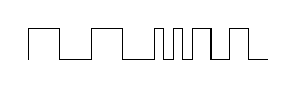
\begin{tikzpicture}[
                              scale=0.4, every node/.style={scale=0.4}
                          ]
                          \draw[yshift=-2] (0,0) -- (0,1) -- (1,1) -- (1,0) -- (2,0)
                          -- (2,1) -- (3,1) -- (3,0) -- (4,0);
                          \draw[yshift=-2, xshift=114, xscale=0.3] (0,0) -- (0,1) -- (1,1) -- (1,0) -- (2,0)
                          -- (2,1) -- (3,1) -- (3,0) -- (4,0);
                          \draw[yshift=-2, xshift=148, xscale=0.6] (0,0) -- (0,1) -- (1,1) -- (1,0) -- (2,0)
                          -- (2,1) -- (3,1) -- (3,0) -- (4,0);
                      \end{tikzpicture}
                \item 440Hz is A4
            \end{itemize}
        \end{column}
        \begin{column}{0.4\textwidth}
            \small
            \centering
            \includegraphics[width=0.4\textwidth]{./images/LK-Buzzer-1.png} \\
            Buzzer\\
            \vspace*{1em}
            \includegraphics[width=\textwidth]{../thesis/images/buzzer-schema.png} \\
            Amplifier Circuit
        \end{column}
    \end{columns}
    % \begin{columns}[T]
    %     \begin{column}{0.5\textwidth}
    %        asdfa 
    %     \end{column}
    %     \begin{column}
    %     \end{column}
    % \end{columns}
\end{frame}


\end{document}
